\documentclass[11pt,a4paper]{article}
\usepackage[margin=25mm]{geometry}
\usepackage[T1]{fontenc}
\usepackage[utf8]{inputenc}
\usepackage{lmodern}
\usepackage{amsmath,amssymb,booktabs,graphicx,hyperref}
\hypersetup{colorlinks=true,linkcolor=blue,citecolor=blue,urlcolor=blue}
\title{Weighted Distribution Aggregation for Heterogeneous Federated Synthetic Data: Bounded Empirical Methods and Results}
\author{Shivansh Gupta\\IIT Guwahati BTP}
\date{25 October 2026}
\begin{document}
\maketitle

\begin{abstract}
We evaluated whether permitted statistical calibration of non-neural client generators improves empirical synthetic-data fidelity over tuned, schema-corrected sample-size weighting while retaining a fixed client-population target. In corrected UCI Adult development, no one of 18 registered three-seed generator/partition/client-count slices achieved the practical 0.005 query-max improvement under the representation constraint; the overall constrained-minus-size difference was $+0.002427903$. The frozen official Adult holdout gave $-0.000214907$ overall, with no one of six slices meeting the margin. A frozen Bank Marketing external-dataset replication gave $-0.001331749$ overall and no one of four practical-gain slices. These are bounded negative comparative findings, not equivalence, population guarantees, or a claim of a new weighting algorithm. The main release is nonprivate.
\end{abstract}

\section{Question and estimand}
For client $i$, let $D_i^{\mathrm{tr}}$ be the real training rows and let $Q_i$ be its locally fitted non-neural joint generator. All clients share the same table schema. The fixed target mass is
\begin{equation}
\alpha_i=\frac{|D_i^{\mathrm{tr}}|}{\sum_j |D_j^{\mathrm{tr}}|}.
\end{equation}
An aggregation rule chooses generator masses $w_i$; changing $w$ does not redefine $\alpha$. For an existing held-out real client reference $D_i^R$, registered bounded query $q$, and generated dataset $D_S$ of exactly $m=10{,}000$ rows, we measure
\begin{align}
b_R(q;\alpha)&=\sum_i\alpha_i\frac{1}{|D_i^R|}\sum_{z\in D_i^R}q(z), &
b_S(q)&=\frac{1}{m}\sum_{z\in D_S}q(z),\\
L_{\mathcal Q}(D_S,D_R;\alpha)&=\max_{q\in\mathcal Q}|b_S(q)-b_R(q;\alpha)|, &
\Delta&=L_{\mathcal Q}(D_S^{\mathrm{challenger}},D_R;\alpha)-L_{\mathcal Q}(D_S^{\mathrm{size}},D_R;\alpha).
\end{align}
Negative $\Delta$ favours the challenger. The ordinary pooled held-out answer is recorded separately. Adult \texttt{fnlwgt} is a predictor, not a survey expansion weight. These are finite-dataset, finite-workload discrepancies, not measured distances between unknown populations or total variation.

\section{Data, generators and access}
Official UCI Adult supplied 32,561 training and 16,281 official-test rows \cite{uci_adult}. Twenty-five official-training rows exactly duplicating official-test records were quarantined. Remaining exact duplicate groups stayed intact across development splitting. Client assignment rules, local tuning and preprocessing were fit from allowed train/local-tune roles and then held fixed. Public numeric support and vocabularies were declared; an Adult education/education-number projection repaired generated rows. A projected discrete joint score requires summing all projection preimages. This was checked for the declared Chow--Liu model; copula and rounded/clipped Gaussian-mixture scores remain approximate.

The corrected Adult development comparison used copula, Chow--Liu and mixed Gaussian-mixture generators, three heterogeneity partitions, $K=5$ and $10$, and seeds 101/202/303: 54 core cells and three independent-marginal controls. Locally selected hyperparameters and fixed checkpoints were reused across weighting rules. Five independent synthetic draws were scored per method/cell. Among the eight candidate statistical families, several require different released information: real-row likelihood evaluations for predictive score, conditional evidence and stacking were privileged evaluator access, whereas summary calibration used declared unnoised aggregate releases. The latter is also nonprivate. Predictive stacking \cite{yao2018stacking}, entropy balancing \cite{hainmueller2012entropy}, kernel matching \cite{huang2009kmm} and private graphical-model measurement fitting \cite{mckenna2019pgm} are prior ingredients, not inventions of this work.

The global generator was selected by mean projected size-weighted \emph{validation} query-max over the same 18 cells per family, averaging five draws within cell. Copula scored 0.029975, Chow--Liu 0.031455 and mixed GMM 0.051446. The complete campaign freeze (full SHA-256 in \texttt{START\_WRITING\_HERE.md}) selected copula with $w=\alpha$, deterministic largest-remainder row counts, the 152-query primary workload and 23-query secondary audit workload. Earlier design choices were assessment-informed, although final family selection used validation only. The official test was first \emph{scored} after this written freeze; raw test records had earlier been read for source validation and duplicate quarantine without method scoring.

\section{Primary fidelity results}
The constrained challenger satisfied $\|w-\alpha\|_1\leq 0.25$ and $w_i\geq 0.5\alpha_i$. The registered practical gain criterion was $\Delta\leq-0.005$ at the declared slice aggregation unit. Corrected Adult development had zero of 18 practical-gain slices and overall mean $\Delta=+0.002427903$. Frozen Adult official-holdout scoring covered 12 cells (three partitions, two values of $K$, seeds 404/505) and five draws for size, uniform and constrained rules in each cell. Mean size loss was 0.022215720, constrained-minus-size was $-0.000214907$, and no one of six two-seed partition/$K$ slices met the practical margin. Frozen official-holdout results were consistent with the bounded development decision to retain size weighting. The same official people recur across all 12 cells; seeds and draws are not independent-person cohorts. Lack of practical gain is neither statistical equivalence nor proof of zero smaller benefit.

The prospectively frozen UCI Bank Marketing external task used the 41,188-row additional-full version and dropped post-contact duration for pre-call prediction \cite{uci_bank_marketing}. Twelve cells spanned two Adult-validation-selected families, two hard skews, $K=5$, and three seeds. Its mean constrained-minus-size difference was $-0.001331749$ with zero of four practical-gain slices. Bank contacts can repeat without person identifiers, so this is cross-dataset replication without a person-independent cohort claim. The transferred numerical margin was an operational choice, not a universal scale of usefulness.

\begin{figure}[ht]
\centering
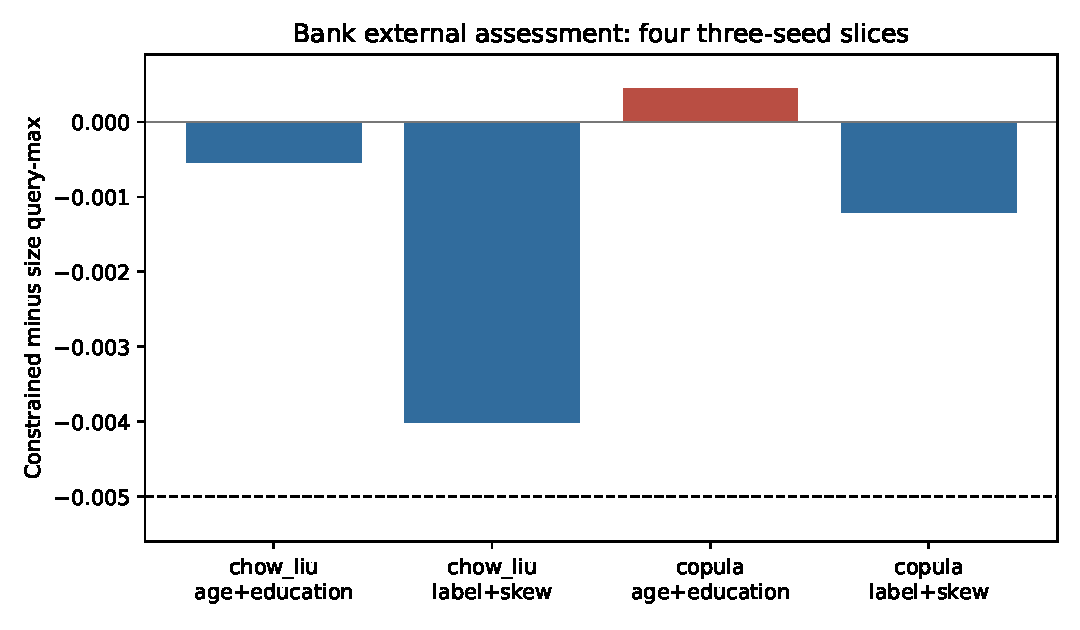
\includegraphics[width=.88\linewidth]{PAPER_FIGURES/bank_external_slice_differences.pdf}
\caption{Bank external replication. Four three-seed slices, with constrained minus size empirical query-max on the vertical axis. The dashed line is the registered $-0.005$ practical margin. No slice met it. The figure was regenerated from saved slice results solely to correct axis-label typography.}
\end{figure}

\section{Mechanisms, utility and conditional fidelity}
Fifty-seven successful fixed-pilot linear programs certified optima only for their finite synthetic query matrices, empirical calibration targets and constraints. Repeated-pilot and synthetic-size analyses separated pilot/draw variability from persistent fitted-model error. Twelve same-row projection checkpoint contrasts, six fixed-pilot summary-access ablations, and six fixed-quantity non-IID severity cells supplied bounded mechanism evidence. Mixtures of overlapping client-subset mixtures algebraically reduce to an effective global mixture; no new within-subset expressive generator is claimed.

The official same-person logistic comparison yielded synthetic-size TSTR Brier 0.129818 and AUROC 0.856167 versus privileged real TRTR Brier 0.101987 and AUROC 0.904646. The \emph{registered budgets differed}: every confirmation cell used 21,148 real training, 4,880 real tuning and 3,254 real calibration rows for TRTR, versus 10,000/2,000/2,000 generated rows for each TSTR rule. No matched-size learning curve was run. These values show performance at registered budgets, not an intrinsic synthetic-data deficit at equal sample size. Extra-trees and supported client/subgroup results are saved separately.

The selected conditional service used a 30,000-row independent teacher support pilot, requiring at least 300 matching rows and 1\% empirical pilot mass, then direct rejection to 1,000 accepted feature rows with a 200,000-proposal cap. Three common registered requests completed in all 12 frozen Adult cells with zero accepted-condition violations; the rare older-doctorate request abstained in all 12. The female-condition mean feature-query maximum was 0.375. Its worst saved query in \emph{every} cell was \texttt{relationship=Husband}: the alpha-standardized real female-conditional frequency was zero in these reference records, while generated frequency ranged from 0.340 to 0.399. This is an observed sex/relationship dependency failure of the frozen model; it does not assert a universal demographic rule. Exact filter satisfaction and pilot support did not ensure fidelity of other features. Trained per-condition Chow--Liu students had separate recorded violations/errors and are not claimed to generalize across arbitrary conditions.

\section{Published references, privacy and limitations}
Four nonprivate same-unnoised-summary Private-PGM fits were a measurement-fitting reference \cite{mckenna2019pgm}; their mean query-max difference from size was $+0.002615$ in the registered development cells. Four adapted FLAIM author-code fits \cite{maddock2024flaim} used interactive raw-client access and private marginals rather than the BTP released-model contract. Their mean difference from a \emph{nonprivate} size utility reference was $+0.012894$, with one favourable cell and three adverse cells. These are protocol-mismatched utility observations, not an equal-privacy ranking. HeteroFedSyn \cite{li2026heterofedsyn} was compared in the access/novelty audit but not numerically reproduced.

Each adapted FLAIM fit reported $(\varepsilon,\delta)=(4,10^{-6})$. If each per-fit guarantee is valid under the stated common adjacency, trust and fixed-membership assumptions, basic sequential composition of all four released fits gives $(\varepsilon_{\mathrm{total}},\delta_{\mathrm{total}})=(16,4\times10^{-6})$ \cite[Theorem~3.16]{dwork2014foundations}. This is approximate-DP accounting for those fits alone. A separate fixed-membership public-bin Laplace histogram at pure-DP $\varepsilon=1,4,8$ has basic composition $\varepsilon=13$ for those releases. Neither protects the unnoised BTP generators, summaries, data-derived partition metadata or full research archive. The main pipeline is \textbf{nonprivate}. In three matched serialized-payload cells, model plus metadata used 1.915--2.866 times the corresponding raw client-table bytes under the same pickle5+gzip6 convention; this is not WAN traffic or a compression claim.

The 152 primary queries can miss unmeasured dependencies. All confirmation configurations reuse official Adult people; Bank may repeat contacts. Five draws estimate synthesis variation conditional on fitted checkpoints and do not constitute independent population replication. Copula nominal ordering, approximate scores, schema projection, finite-pilot error and severe within-condition failure limit broader claims. The supported thesis contribution is a reproducible comparative negative result, explicit target/representation accounting, support-aware diagnostics, and a justified size-weight fallback. General superiority, whole-pipeline privacy, arbitrary-condition fidelity, a novel theorem and publication readiness remain unestablished.

\section*{Author's theory and discussion placeholders}
Add the formal finite-sample fallback proposition and representation-bound counterexamples. Characterize projected pushforward probabilities and support-dependent conditional transfer, following \texttt{THEORY\_ONLY\_BACKLOG.md}. Discuss when stronger local models reduce weighting headroom. Distinguish observed datasets from population claims. No new experimental result is required for the bounded empirical statement above.

\begingroup\small
\bibliographystyle{plain}
\bibliography{references}
\endgroup
\end{document}
